\section{Baseline Platform}

\begin{frame}{Baseline Platform - Hardware}
    \centering 2D-mesh, credit-based, wormwhole, XY routing, manycore
    \begin{figure}[!ht]
       \centerline{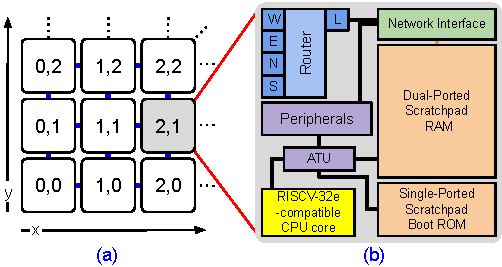
\includegraphics[width=.6\columnwidth]{fig/soc.pdf}}
    \end{figure}    
\end{frame}

\begin{frame}{Baseline Platform - Hardware (contd.)}
	\begin{itemize}
		\item Network interface (NI) allows for DMA (like ~\cite{Ruaro2019Memphis,ruaro_dmni})
		
		\item CPU get interrupted by the NI once a packet is entirely received
		
		\item Sending a packet follows a similar strategy, where the network device driver configures the NI to copy the packet from RAM into the local port of the router. 
		
		\item At the kernel level, the network driver has a queue of packets, where the NI stores packets. Tasks can probe the driver for packets or perform a self-blocking operation until a packet is received. The driver also allows tasks in the same PE to communicate by moving packets between queues.%GRAMMARLY-O
	\end{itemize}
\end{frame}


\begin{frame}{Baseline Platform - Software}
    \begin{itemize}
        \item PEs run the UCX-OS~\cite{ucxos:2024} kernel
        \item Priority-based round-robin (PBRR) technique~\cite{Nithya:2023}
        \item Accounts for dependency. The kernel keeps track of the number of iterations of tasks as new packets arrive, prioritizing (i) tasks in the oldest iterations and (ii) tasks meeting their data dependencies in case of a tie.
    \end{itemize}
\end{frame}
